%                                                                                          \color{cyan} %color de texto con 70-80 % o más de avance
\section{Introducción}
%\subsection{Fotointerpretación}
Como fue señalado en el capitulo anterior, esta tesis concentra su aporte en herramientas para el monitoreo remoto de bosques nativos.
Es un proceso que se enmarca en la teledetección, y de forma más específica, en la fotointerpretación. Esta consiste en el análisis de imágenes aéreas sobre un terreno, para extraer información, identificar objetos o clasificarlos, entre otros fines. 
Durante un tiempo la fotointerpretación era llevada a cabo de manera manual, valiéndose el fotointerpretador de una imagen impresa y herramientas como estereoscopio, reglas y marcadores, mediante las cuales realizaba la identificación de objetos en la imagen \cite{noauthor_teledeteccion_nodate,hernandez_tecnologias_2011,garcia_introduccion_nodate}. Con la mayor accesibilidad y disponibilidad de herramientas digitales, se vuelve más atractivo el uso de métodos que automaticen la tarea, optimizando el tiempo y potenciando así las aplicaciones.

En el caso de las imágenes aéreas es muy probable que sean necesarias varias imágenes para cubrir la zona de interés. Así, el punto de inicio es la captura de fotogramas mediante alguna plataforma que puede ser una aeronave o un satélite. A partir de una cantidad considerable de imágenes se compone lo que se conoce como ortomosaico \cite{liba_accuracy_2015}. Para el mismo se recomienda garantizar al momento de realizar las capturas  un mínimo nivel de solapamiento entre imágenes consecutivas y entre aquellas que pertenecen a líneas de vuelo adyacentes. En capturas relacionadas con imágenes de bosques nativos es necesario un nivel alto de solapamiento, llegando al 85\% frontal y 70\% en el lateral \cite{sestari_rpas_2019,dandois_optimal_2015,seifert_influence_2019}. Esto se debe a la compleja geometría que se observa en las imágenes, que incluyen miles de ramas y hojas distribuidas de forma irregular. Otra recomendación es aumentar la altitud de vuelo \cite{bhatt_image_2022}. Al volar más alto, las imágenes sufren menos distorsiones de perspectiva y es más fácil detectar similitudes visuales entre las imágenes superpuestas en áreas de vegetación.

A continuación, se abordarán en detalle el marco teórico de los dos puntos en los que esta tesis hace sus principales aportes, que son las plataformas de sensado remoto y el procesamiento automático de las imágenes.

\subsection{Plataformas para el sensado remoto}
En este apartado se exponen las principales características de las opciones de plataformas para el sensado remoto, agrupadas en satélites artificiales, aeronaves tripuladas y no tripuladas.
\subsubsection{Satélites}

Se entiende por satélite artificial a todo dispositivo fabricado por el ser humano que es puesto en órbita alrededor del planeta Tierra con diversos propósitos, destacándose el establecimiento de comunicaciones y la observación terrestre por medio del sensado remoto. Éste último es el que reviste interés para el presente trabajo. Los satélites para sensado remoto van generalmente equipados con sensores multiespectrales, de múltiples bandas. La operación de los satélites es de manera continua desde que son puestos en órbita hasta el fin de su vida útil. El lanzamiento y puesta en órbita requiere de infraestructura adecuada a tal fin, de las cuales hay muy pocas en el mundo, concentradas en no más de una decena de países \cite{noauthor_que_nodate}. Para poner un satélite en órbita, la cual suele situarse a kilómetros de la corteza terrestre, el mismo requiere ser lanzado por medio de un vehículo espacial, generalmente un cohete, ya que no tiene propulsión propia que le permita despegar y alcanzar la altitud de órbita. Una vez allí, por el propio fenómeno de interacción gravitacional con la Tierra, se desplaza alrededor del planeta.
Los datos recopilados por los satélites son transmitidos a estaciones terrenas ubicadas en distintos puntos del planeta, y el acceso a las imágenes de alta resolución suele ser restringido a una contraprestación monetaria. No obstante suele haber acceso gratuito a imágenes con menor resolución, que para las imágenes satelitales son de cuatro tipos: resolución espacial, espectral, temporal y radiométrica.

Al cabo de su vida útil, la cual transcurre entre cinco y quince años, el satélite precipita hacia la Tierra, o se posicionan en órbitas destinadas a ese fin \cite{noauthor_keeping_nodate}. Algunos satélites están equipados con un sistema de control de posicionamiento que mantiene y corrige si es necesario los parámetros de órbita.

Según la base de datos de la Unión de Científicos Conscientes \cite{noauthor_satelites_nodate}, actualizada el primero de mayo de 2.022, existen alrededor de 5.500 satélites orbitando la Tierra, de los cuales 1.156 (un 21\%) tienen por finalidad la observación terrestre. En la tabla \ref{Satelites} se describen las características de los satélites más reconocidos, como ser tamaño de imagen, resoluciones espaciales, radiométricas y temporales. 

Los sensores utilizados pueden ser de varios tipos, considerando el rango de frecuencias o la longitud de onda para cuya adquisición han sido diseñados. Se destacan los de luz visible, infrarrojo cercano (\textit{near infrared} - NIR), infrarrojo térmico (\textit{thermal infrared} - TIR), pancromático e infrarrojo de onda corta (\textit{shortwave infrared} - SWIR). También existe un considerable despliegue de radares de apertura sintética (\textit{synthetic aperture radar} - SAR) en diferentes bandas. De los satélites de observación terrestre, aproximadamente un 40\% son con sensores ópticos, es decir, capturan imágenes en el espectro visible.

Hay muchas y muy diversas fuentes de imágenes satelitales, tanto en forma gratuita como pagas. Entre las opciones pagas, imágenes multiespectrales con una resolución espacial de 50 cm se consiguen por montos entre 10 dólares por km\textsuperscript{2} hasta 29 dólares por km\textsuperscript{2} según sean actualizadas o de archivo (generalmente más de 90 días)\cite{noauthor_satellite_2020}. Debe tenerse en cuenta el tamaño mínimo del área a ser adquirida, en caso de las imágenes de archivo son 25 km\textsuperscript{2} (2.500 ha) y las actualizadas son de 100 km\textsuperscript{2} (10.000 ha).
\begin{table}[H]
    \centering
    \caption{Características de sensores satelitales. Fuente \cite{noauthor_3_nodate}}
    \begin{tabular}{c p{20mm} p{15mm} p{15mm} p{25mm} p{20mm}p{20mm} p{20mm}|}
        \hline
        \hline
        \textbf{Sensor} & \textbf{Tamaño de imagen} & \multicolumn{4}{c}{\textbf{Resolución}} & \textbf{Aplicación principal} \\
        %\hline
        & & \textbf{Espacial} & \textbf{Temporal} & \textbf{Radiométrica} & \textbf{Espectral}  &\\
        \hline \hline
        Meteosat & Toda la esfera & 	2500 m 	& 0.5 h 	& 256 ND 	& 1Vis 1IR 1 IT & Meteorología\\
        \hline
        NOAA AVHRR & 2700 x 2700 km	& 1100 m 	 	& 12 h 	& 1024 ND 	& 2Vis 1IR 1IT & Observación atmosférica\\
        \hline
        Landsat TM 	& 185 x 185 km & 30 m 	 	& 16 d 	& 256 ND 	& 3Vis 3IR 1IT & Observación terrestre\\
        \hline
        SPOT HRV & 60 x 60 km	& 20 m 	 	& 20 d	& 256 ND 	& 2Vis 1IR & Observación terrestre\\
        \hline
        SPOT Vegetation & 2200 x 200 km	& 1150 m 	 	& 1 d	& 1024 ND 	& 2Vis 2IR & Monitoreo agrícola\\
        \hline
        MODIS & 2330 x 2330 km	& 250 - 100 m 	 km 	& 1 d	& 1024 ND 	& 36 bandas & Observación terrestre\\
        \hline
        IKONOS & 100 x 100 km	& 4 m 	 	& 3 d 	& 2048 ND 	& 3Vis 1IR & Observación terrestre\\
        \hline
        Albedo & 35 x 7 km & 0,4 m  & 1 d & S/D & 3Vis 1IR & Observación terrestre\\
        \hline
         Worldview & 13 x 13 km &   & 1 d & 2048 & 29 bandas & Observación terrestre\\
        \hline
         Sentinel & 13 x 13 km &  10 m & 1 d & S/D & 13 bandas & Observación terrestre\\
        \hline
        \hline
    \end{tabular}

\label{Satelites}
\end{table}

Además de la erogación requerida para adquirir imágenes satelitales, su análisis es una tarea costosa y laboriosa que exige inversiones importantes de tiempo, considerando que pueden ser miles de imágenes de alta resolución, demandando recursos informáticos y expertos en sistemas de información geográfica (SIG). Si bien existen plataformas en línea que proporcionan datos y herramientas para el monitoreo de bosques, como \textit{Global Forest Watch}, aún carecen de flexibilidad y de imágenes de alta calidad, factores indispensables para mostrar los cambios ocurridos en mayor detalle.


\subsubsection{Aeronaves}
Otro tipo de plataforma para realizar el sensado remoto son las aeronaves, tripuladas o no. A diferencia de los satélites, las aeronaves no salen de la atmósfera, y la altitud de vuelo puede alcanzar los 15.000 metros sobre el nivel del mar. Las imágenes aéreas se toman mediante sensores montados en la estructura de la aeronave. La misión de captura de imágenes por medio de aeronaves se definen para un vuelo específico. Eso conlleva otros tiempos diferentes a las misiones satelitales, ya que implica programar y preparar el vuelo, y eventualmente trasladar la aeronave. Entre las variables que intervienen en la duración del vuelo en la fase de captura de imágenes se puede mencionar la extensión del área de interés, la velocidad de desplazamiento y la altura de vuelo. Esto también tendrá incidencia en la resolución espacial de las imágenes y en el espacio de almacenamiento requerido.

%\begin{figure}
%    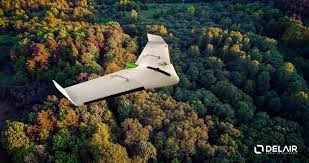
\includegraphics[width=0.3\textwidth]{Imagenes/dron.jpg}
%     \hfill
%     \caption{Acá puede ir o no una imagen ilustrativa; revisar que esté referenciada correctamente}
%    \label{dron}
%\end{figure}
%\paragraph{Aeronaves convencionales tripuladas}
A esta sección corresponden las aeronaves de mayor porte, cuya operación debe hacerse con tripulación, requiriendo que sea personal capacitado y con licencia para operarlas. En esta categoría se incluyen los aviones de ala fija, los de ala rotatoria (helicópteros) así como aerostatos. Su operación requiere de una planificación de vuelo que debe ser reportada al área de espacio de vuelo controlado, además de necesitar una base de despegue y aterrizaje, así como de traslado al aeródromo del cual despega y al cual regresa para aterrizar.   Finalmente en el costo total del procedimiento, en el caso de aeronaves tripuladas, incidirá el tiempo que lleve desde la puesta en marcha del motor hasta su apagado, ya que todo eso se contempla como hora de vuelo.
El marco regulatorio de estas operaciones son las Regulaciones Argentinas de la Aviación Civil (RAAC), Parte 91 \cite{noauthor_infoleg_nodate-1}. 


\paragraph{Aeronaves no tripuladas}
Los vehículos aéreos no tripulados (VANT), también conocidos en la literatura como sistemas aeros no tripulados (\textit{Unmanned Aerial Systems} - UAS) son cada vez más asequibles por el público general. Disponibles en amplia variedad de modelos, constituyen una formidable herramienta para llevar a cabo tareas de relevamiento aéreo. El abanico de posibilidades se ve ampliado por prescindir de una pista de despegue o aterrizaje de dimensiones grandes. El marco legal regulatorio para la actividad con VANT es la resolución ANAC 885 \cite{noauthor_infoleg_nodate}.

Existe una amplia variedad de tipos de VANT, que pueden ser de múltiples rotores o de ala fija. El presente trabajo no es exhaustivo en este aspecto, pero a los efectos de describir las características principales, se lo hará con algunos de ellos.
\subparagraph{Multirrotor}
Los VANT tipo multirrotor poseen cuatro o más hélices para proporcionar al vehículo la sustentación y la propulsión en tres ejes de desplazamiento. Esta característica es la que le confiere mayor maniobrabilidad, especialmente en espacios reducidos. La energía para propulsarse es eléctrica, proveniente de baterías. Son los más difundidos comercialmente. Algunos ejemplos son:
\begin{itemize}
    \item DJI Mini 2:\\
    Un dron comercial asequible del fabricante DJI \cite{noauthor_dji_nodate-1}. Está equipado con una cámara con sensor 1/2.3” CMOS, de 12 millones de píxeles efectivos. La lente de la cámara posee un ángulo de visión de 83º y un formato equivalente a 35 mm de longitud focal de 24 mm, una apertura de f/2.8 y un rango focal de 1 m hasta infinito. En cuanto a las velocidades, el dron tiene tres modos de funcionamiento, modo deportivo o rápido (Sport), modo Normal y modo de vuelo lento (Cine). En Sport se desplaza hasta 16 m/s, en modo normal 10 m/s y en modo cine 6 m/s.
    \item DJI Mavic 3M:\\
    Este es un dron profesional \cite{noauthor_dji_nodate}. Cuenta con una cámara RGB de 4/3 CMOS, con 20 millones de píxeles efectivos. La lente es de un campo de visión de 84º, con una longitud focal equivalente de 24 mm. La apertura es de f/2.8 a f/11, y foco de 1 m al infinito. En modo normal puede desplazarse hasta 15 m/s.
\end{itemize}

\subparagraph{Ala fija}
Este tipo de VANT poseen un ala fija que le brinda sustentación, por lo que pueden incluso planear aunque falle la planta motriz de la aeronave. Sus características de funcionamiento permiten vuelos más extensos, cubriendo mayores áreas. Existen VANT de ala fija alimentados eléctricamente con baterías o con motores de combustión interna. Se los encuentra esencialmente en aplicaciones de agricultura de precisión y en el campo militar. Un ejemplo es Asesor/9, que es un VANT de ala fija de casi 2 m de envergadura \cite{noauthor_drone_nodate}. Puede desplazarse a 17 m/s y tiene una autonomía de dos horas de vuelo. Va equipado con una cámara multiespectral MicaSense Altum-PT \cite{noauthor_altum-pt_2023} cuyo sensor es de 12,4 millones de píxeles, que le confieren una resolución de 5,28 cm/pixel volando a 120 m sobre el terreno.

\subsection{Sensores}
En el sensado remoto, los elementos clave para llevar a cabo la tarea son los sensores. Estos constituyen la carga útil de las plataformas de sensado remoto, y pueden ser de distinto tipo.
Los sensores remotos que serán tratados en el presente trabajo son del tipo pasivo, es decir, están compuestos por detectores que registran las ondas de luz solar reflejadas en el terreno. Particularmente nos interesan, por una cuestión de costos, los que cubren el espectro visible. Básicamente constituyen una cámara fotográfica, que se compone de un arreglo de lentes y espejos que refractan y reflejan la luz, proyectándola sobre un sensor fotosensible, generalmente es un rectángulo conformado como un arreglo de detectores, cada uno de ellos representa a un pixel de la imagen. La resolución espacial de la imagen queda determinada por las características constructivas de estos sensores y la configuración de lentes, y la distancia al objetivo. 
 La distancia focal es un atributo de cada cámara. El factor de escala está dado por la altura de vuelo sobre el terreno, que puede variar incluso durante el vuelo, y por la distancia focal de la cámara, que es fija. 
 Algunas características de sensores de cámaras fotográficas que se consiguen en el mercado se exponen a continuación.

%12.4 MP sensor pancromático
%Cinco bandas espectrales de 3.2 MP
%Resolución Multiespectral (pan-sharpened): 1.24cm/pixel a 60m; 2.49cm/pixel a 120m

%RGB 12.4 MP (obturador global, alineado con todas las bandas)
%Sensor térmicoFLIR LWIR infrarrojo térmico 7.5-13.5um calibrado radiométricamente
%RESOLUCIÓN5.28 cm cm / pixel (por banda MS), 33.5 cm / pixel (banda térmica), 2.49 cm / pixel (pancro) a 120 m AGL
%VELOCIDAD DE CAPTURA Hasta 3 capturas por segundo DNG sin procesar
%INTERFACES3 GPIO: señal de disparo, salida de la parte superior del cuadro, salida de 1 PPS, botón host. Puerto USB 2.0 para WiFi, ethernet 10/100/1000, serial, y almacenamiento CFexpress
%CAMPO DE VISIÓN50° HFOV x 38° VFOV (MS) / 44° HFOV x 38° VFOV (PAN)
\color{black}

\subsubsection{Cámaras fotográficas}
Los equipos de fotografía que suelen usarse en las plataformas aéreas varían de acuerdo con especificaciones y aplicaciones. Las cámaras que van montadas en aeronaves convencionales suelen ser de mayor tamaño, y van fijadas en el fuselaje. Un ejemplo de este tipo de cámaras es la Vexcel \cite{noauthor_ultracam_nodate}, cuyo peso es de 60 kg. Esta cámara es de cuatro bandas, correspondientes al rojo, verde, azul e infrarrojo cercano. En las aeronaves no tripuladas las cámaras pueden ser de diversos tipos, inclusive puede adaptarse prácticamente cualquier tipo de cámara comercialmente disponible a un soporte fijado al VANT. Como el uso de cámaras en drones está bastante extendido en el ámbito de relevamiento y monitoreo aplicado en la agricultura, es común encontrar cámaras cuyas especificaciones espectrales abarquen el infrarrojo, o el borde rojo, además del espectro visible. Un ejemplo es la cámara Micasense \cite{noauthor_altum-pt_2023}, con siete bandas, las cuales son rojo, verde, azul, infrarrojo cercano, borde rojo, pancromático y térmico.
 %https://www.vexcel-imaging.com/brochures/UC_Eagle_4.1_es.pdf
 %https://ageagle.com/wp-content/uploads/2022/07/AgEagle-Altum-PT-Brochure-EN.pdf
 
%Se podría añadir como figura un mapa con las regiones de información de vuelo (FIR), con las zonas de control, aeródromos habilitados, por ejemplo, etc.
\subsection{Plataformas y Sensores Utilizados en el Monitoreo de Áreas Forestales}

Describir los estudios encontrados principalmente entre 2018, 2019 y Bhatt 2022 
Los costos y flexibilidad han permitido de los VANT sean una de las plataformas preferidas para una serie de aplicaciones relacionadas con el monitoreo de áreas preservadas, como monitoreo y manejo de la vida silvestre, monitoreo de ecosistemas, ecoturismo, gestión ambiental,  gestión de crisis asociadas a desastres ambientales, entre otras \cite{jimenez_lopez_drones_2019}.
Algunos autores han identificado aspectos negativos del uso de drones en la conservación \cite{jimenez_lopez_drones_2019}. Es necesario investigar más a fondo los posibles efectos de perturbación en la vida silvestre \cite{millner_between_2024}. El uso de drones como herramientas de coerción podría debilitar el compromiso ambiental de las comunidades en áreas protegidas \cite{sandbrook_social_2015}, y por lo tanto, podría resultar contraproducente para la conservación. Por otro lado, la enorme cantidad de datos adquiridos con drones requiere métodos modernos, robustos y computacionalmente intensivos para derivar información precisa y significativa \cite{manfreda_use_2018}, lo que puede representar una barrera tecnológica para el uso efectivo de esta tecnología en áreas protegidas.

\section{Procesamiento Automático de Imágenes}

En esta sección se expondrá el marco teórico que sustenta las contribuciones de esta tesis en relación al procesamiento automático de imágenes aéreas. Comenzando por algunas definiciones elementales.

\subsection{Imagen Digital}
Con los dispositivos de carga acoplada (\textit{Charge-Coupled Device} - CCD), que capturan la luz en forma de cargas eléctricas para luego ser convertidas en una señal digital, surgieron las primeras cámaras digitales \cite{dyck_chapter_1982}. Posteriormente los sensores con semiconductor complementario de óxido de metal (\textit{Complementary Metal-Oxide-Semiconductor} - CMOS) simplificaron el proceso de obtener imágenes, convirtiendo directamente luz en señal digital, reduciendo el consumo energético y abaratando costos, consolidando definitivamente la popularidad de las cámaras digitales \cite{fossum_cmos_1997}. Desde entonces, una imagen se convirtió en una matriz (o conjunto de matrices) de dígitos binarios.

Los elementos que componen la imagen digital se denominan píxeles, y desde el punto de vista algebraico, son los elementos de una matriz de ancho \textit{N} y alto \textit{M} determinados. A su vez cada píxel está caracterizado por composición de bandas o canales. Si la imagen es de color en espectro visible existen tres canales o bandas correspondientes al rojo (dentro del rango de 645-700 nm), verde (en el rango de 500-550 nm) y azul (alrededor de los 470 nm) (ver figura \ref{RGB}), también conocido con el acrónimo RGB (\textit{Red}, \textit{Green} y \textit{Blue} en inglés. La combinación de las características de cada canal o banda constituirá el color con el que se percibe el píxel. De modo que si cada banda se representa con un ancho de palabra de ocho bits, se establecen 256 niveles distintos (equivalente a ($2^8$)), resultando en que cada píxel puede adoptar hasta más de 16 millones de colores.


\begin{figure}[h!]
    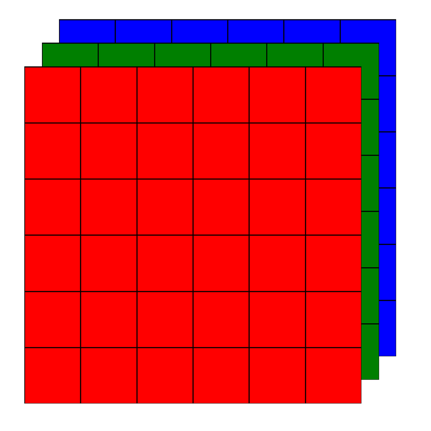
\includegraphics[width=0.3\textwidth]{Imagenes/imagen-a-color.png}
     %\hfill
     \caption{Composición de imagen a color en tres canales, rojo, verde y azul (fuente: https://www.codificandobits.com/blog/convolucion-redes-convolucionales/)}
    \label{RGB}
\end{figure}

La imagen como matriz porta consigo información que puede ser procesada y analizada por variados métodos, dependiendo del tipo de imagen y de información que se busca extraer. En general, previo al análisis de imágenes se suele aplicar un preprocesamiento que involucra algún tipo de filtrado, o algún ajuste de parámetros de la imagen, como el contraste o ecualizado de bandas \cite{sonka_image_1993}. También suele realizarse alguna conversión entre diferentes espacios de color, según los requerimientos.\\

Con frecuencia son de utilidad los histogramas de las imágenes, los cuales consisten en ordenar los niveles de intensidad por canal o banda y graficar la cantidad de píxeles por cada nivel \cite{atienza_histograma_nodate}. También desde el aspecto morfológico es posible efectuar el análisis de imágenes estudiando cada pixel y sus alrededores, examinando la estructura de la imagen. De ese tipo de análisis surge la identificación de formas y texturas.

Con otro tipo de enfoques es posible analizar las imágenes en elementos más sutiles o complejos, como puede ser la presencia de sombras. Se puede suponer que los píxeles que corresponden a sombras son más oscuros que los otros, es decir, el valor de la intensidad del pixel es menor, pero en la realidad esto no es así, por lo que es necesario usar otras metodologías. 
Se podría decir que en esta tesis se analizan varios niveles de detalle en las imágenes, como la detección de sombras \cite{bernhardt_identification_2023}, y la identificación de copas \cite{hubert_wagner_individual_2018}.
En las secciones siguientes, se profundiza en el estado el arte de la detección de estos elementos.

\subsection{Sombras en dosel selvático}
La presencia de sombras en las imágenes aéreas puede ser de ayuda en el análisis de la estructura del dosel selvático, al aportar información sobre la eventual existencia de ejemplares de capa emergente. Asimismo puede ser un signo descriptivo de la estructura de la porción de selva estudiada, evidenciando claros en la selva que denoten algún tipo de acción extractiva, o la presencia de áreas degradadas o con flora de soto bosque nativo o exótico amenazantes \cite{bedrij_selective_2022}.

Para detectar sombra, es posible basarse en el modelo Stockham \cite{stockham_image_1972}, según el cual una imagen puede descomponerse en dos partes, una la denominada iluminación y la otra componente es la reflexión. Llevadas al plano de frecuencias, se confirma el hecho de que la componente de iluminación tiene una variación más lenta, es decir, se corresponde con las frecuencias bajas. De modo similar, la componente de reflexión se corresponde con frecuencias altas \cite{oppenheim_nonlinear_1968}. Entendiendo esto, es factible implementar un filtrado en la imagen para realzar las sombras, separando la componente de iluminación de la de reflexión. Esta técnica fue utilizada en la remoción de sombras en imágenes de piezas de manufactura \cite{yang_research_2012} y en la detección automática de sombras en objetos oscuros \cite{etemadnia_automatic_2003}. En el presente trabajo, la aplicación en análisis de la estructura de la selva es novedosa.


%\subsubsection{C1-Lógica difusa y procesamiento homomórfico (sombras)}
\subsection{Conteo de Copas}
El tratamiento automático de clasificación de especies arbóreas a partir de imágenes requiere de un conjunto de habilidades informáticas que van desde la manipulación el tratamiento de las imágenes hasta el entrenamiento de modelos de aprendizaje automático. Para obtener una aceptable clasificación de copas es necesario realizar procesamiento a la imagen aprovechando las características de textura y contraste que ésta exhibe. Los algoritmos propuestos en la literatura posibilitan una adecuada segmentación de las copas individuales del dosel y capa emergente de la Selva Atlántica en imágenes satelitales hiperestectrales \cite{ferreira_tree_2019}, lo que consecuentemente habilita en otro nivel la clasificación por especies. 

En esta tesis se utiliza como base la propuesta \cite{ferreira_tree_2019} para evaluar su potencial aplicación en el análisis de imágenes aéreas de la selva atlántica en la provincia de Misiones.
Partiendo de una imagen en escala de grises, se realiza una secuencia de pasos en los que se implementan diferentes filtros para identificar cada una de las copas, de un modo que finalmente se obtuvo una imagen binarizada con la cual se pudo obtener un conteo de las copas. El primer paso consiste en hacer una clara identificación de los bordes y del área de copas. Luego se aplica un algoritmo de Rolling Ball \cite{sternberg_biomedical_1983} que produce un suavizado en los niveles de grises dentro de las copas. En una siguiente etapa, distinguiendo copas grandes de pequeñas, se identifican huecos en las copas grandes, para posteriormente rellenarlos con un valor promedio. Una vez rellenos todos los huecos y uniformadas todas las copas, se procede a segmentarlas, obteniéndose una imagen binarizada, con cada copa de árbol aislada e identificada en su posición.

